\documentclass[11pt]{article}
\usepackage[margin=1in]{geometry}
\usepackage{graphicx}
\usepackage{booktabs}
\usepackage{caption}
\usepackage{natbib}
\usepackage{hyperref}

\title{Early Pregnancy Gene Expression, Vitamin D Status, and Preeclampsia}
\author{Tanner Rougeau}
\date{\today}

\begin{document}
\maketitle

\section{Methods}

\subsection{Data Source}
Data came from the publicly available Gene Expression Omnibus dataset GSE85307, which was generated as part of a nested case-control study within the Vitamin D Antenatal Asthma Reduction Trial (VDAART) \citep{mirzakhani2016}. The study measured gene expression in peripheral blood collected early in pregnancy (10 to 19 weeks of gestation) using the Affymetrix Human Gene 1.0 ST Array. The initial sample included 157 women, 47 of whom developed preeclampsia and 110 of whom had normal pregnancies. For this project, I used a subset of 500 probes along with covariate data on maternal age, BMI, vitamin D, asthma status, gestational age at delivery and at sample collection, and microarray batch.

\subsection{Data Processing}
All data wrangling was completed in R. Covariate values were stored as text with descriptive labels attached, so I removed the labels and converted each variable to numeric or categorical format. Probe IDs were matched to gene names using the provided linker file, and expression data were matched to covariate data by GEO sample ID. I verified that all 157 expression samples had a matching covariate record and vice versa. No covariate values were missing or implausible, so no participants were excluded and the final sample size remained 157. I created a categorical vitamin D variable by classifying women as deficient ($<$20 ng/mL) or sufficient ($\geq$20 ng/mL). I chose 20 ng/mL because it is a commonly used clinical threshold for deficiency and it divided the sample into groups of similar size (median 20.4 ng/mL), although the original study defined sufficiency as $\geq$30 ng/mL \citep{mirzakhani2016}.

\subsection{Statistical Analysis}
To select genes for visualization, I compared mean expression between women with preeclampsia and women with normal pregnancies for each of the 500 genes using Welch's two-sample t-test and ranked genes by p-value. Because this screen involved 500 tests without correction for multiple comparisons, it was treated as exploratory. I selected \textit{RUNDC3A} for detailed plotting because it had the largest mean difference among the ten top-ranked genes, and the ten top-ranked genes were used for the heatmap. Summary statistics were stratified by preeclampsia status and reported as mean (SD) for approximately normal continuous variables, median [IQR] for skewed continuous variables, and n (\%) for categorical variables. For \textit{RUNDC3A}, I plotted the distribution of expression with a histogram, its relationship with maternal BMI with a scatterplot and fitted linear regression line, and its distribution by pregnancy outcome and vitamin D status with a boxplot overlaid with jittered points to show group sizes. A random seed was set so jittered point positions were reproducible. The heatmap of the ten top-ranked genes used row-scaled (z-score) expression with hierarchical clustering of genes and samples (Euclidean distance, complete linkage) and tracking bars for pregnancy outcome and vitamin D status. Finally, I used a beeswarm plot to show the mean difference in expression between groups for all 500 genes, highlighting genes with p $<$ 0.05.

\subsection{Software}
All analyses were performed in R version [X.X.X] \citep{R-base}. Data wrangling used tidyverse version [X.X.X] \citep{R-tidyverse}, and figures were created with ggplot2 version [X.X.X] \citep{R-ggplot2}, ggpubr version [X.X.X] \citep{R-ggpubr}, pheatmap version [X.X.X] \citep{R-pheatmap}, and ggbeeswarm version [X.X.X] \citep{R-ggbeeswarm}. Reports were generated with knitr version [X.X.X] \citep{R-knitr}. All code is available at \url{https://github.com/tannerrougeau/QBS103-FinalProject}.
\section{Results}

\subsection{Study Population}
Of the 157 women included, 47 (29.9\%) developed preeclampsia (Table~\ref{tab:summary}). Maternal age was similar between groups (mean 26.6 years in normal pregnancies vs. 25.8 years in preeclampsia). Women who developed preeclampsia had higher BMI (median 31.2 vs. 26.5 kg/m$^2$). Median gestational age at delivery was similar (39.1 vs. 39.3 weeks), although the lower quartile was earlier in preeclampsia (36.9 vs. 38.6 weeks), suggesting more early deliveries in this group. Vitamin D deficiency was somewhat more common in women who developed preeclampsia (55.3\% vs. 47.3\%; Table~\ref{tab:summary}).

\begin{table}[htbp]
\centering
\caption{Characteristics of the study population stratified by pregnancy outcome. Continuous variables are reported as mean (SD) or median [IQR], and vitamin D status as n (\%), with deficiency defined as $<$20 ng/mL.}
\label{tab:summary}
\resizebox{\textwidth}{!}{%
\begin{tabular}{llll}
\toprule
  & Normal (n = 110) & Preeclampsia (n = 47) & Overall (n = 157)\\
\midrule
Maternal age (years), mean (SD) & 26.63 (5.08) & 25.78 (4.95) & 26.38 (5.04)\\
Maternal BMI (kg/m$^2$), median [IQR] & 26.54 [22.35, 30.97] & 31.24 [24.62, 36.41] & 27.33 [22.9, 33.27]\\
Gestational age at delivery (weeks), median [IQR] & 39.29 [38.57, 40] & 39.14 [36.93, 40.07] & 39.29 [38.14, 40]\\
Vitamin D status, n (\%) & Sufficient: 58 (52.7), Deficient: 52 (47.3) & Sufficient: 21 (44.7), Deficient: 26 (55.3) & Sufficient: 79 (50.3), Deficient: 78 (49.7)\\
\bottomrule
\end{tabular}
}
\end{table}

\subsection{\textit{RUNDC3A} Expression}
\textit{RUNDC3A} expression was approximately normally distributed, centered near 9 on the log$_2$ scale, with no extreme outliers (Figure~\ref{fig:rundc3a}A). Expression was not associated with maternal BMI, as the fitted regression line was nearly flat across the range of BMI values (Figure~\ref{fig:rundc3a}B). Women who developed preeclampsia had slightly lower median \textit{RUNDC3A} expression than women with normal pregnancies in both vitamin D groups, although the distributions overlapped considerably and vitamin D status showed little difference within each outcome (Figure~\ref{fig:rundc3a}C).

\begin{figure}[htbp]
\centering
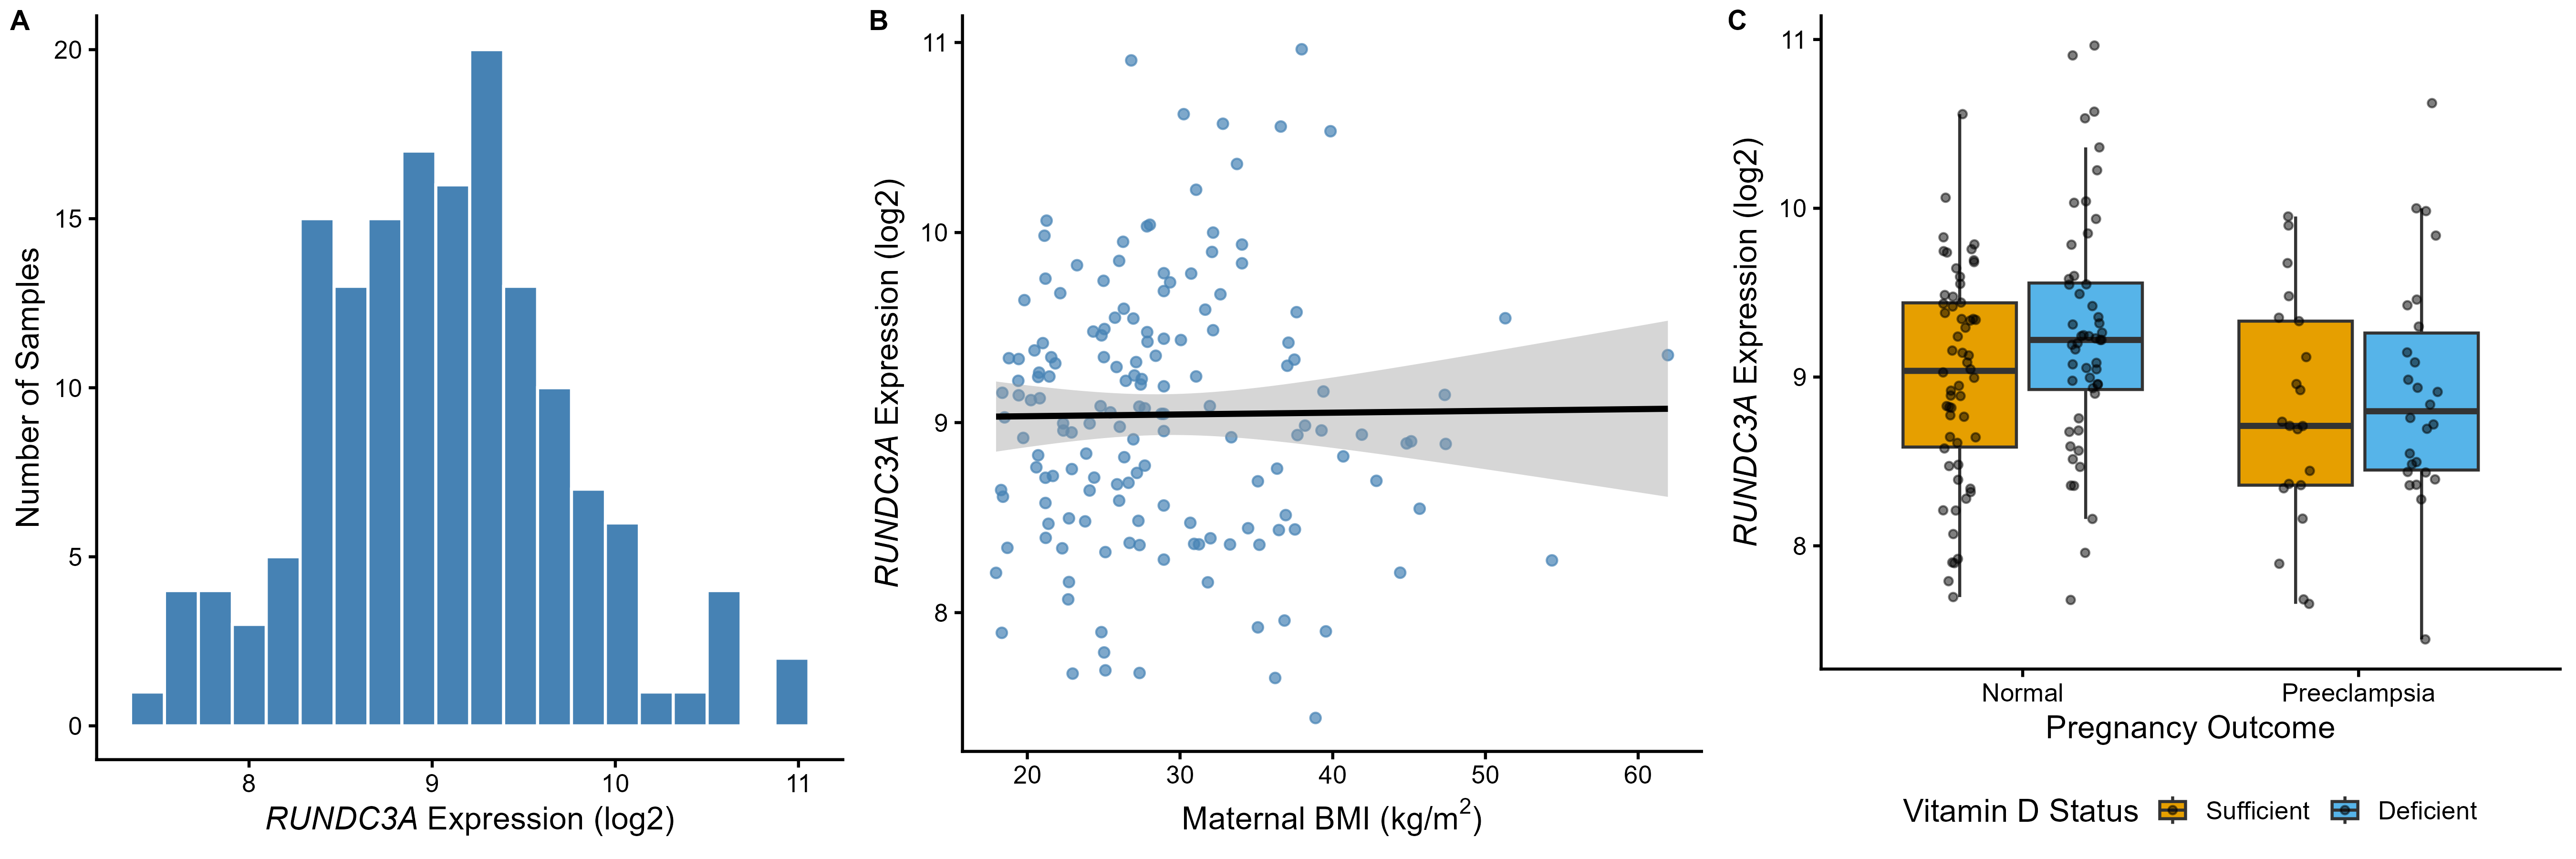
\includegraphics[width=\textwidth]{RUNDC3A_panel.png}
\caption{\textit{RUNDC3A} expression in early pregnancy. (A) Distribution of log$_2$ \textit{RUNDC3A} expression across all 157 women. (B) \textit{RUNDC3A} expression versus maternal BMI with a fitted linear regression line and 95\% confidence band. (C) \textit{RUNDC3A} expression by pregnancy outcome and vitamin D status, with jittered points showing individual women.}
\label{fig:rundc3a}
\end{figure}

\subsection{Top-Ranked Genes}
The ten genes with the smallest p-values clustered into two groups that corresponded to the direction of their difference: \textit{RUNDC3A}, \textit{YIPF6}, and \textit{MOSPD1}, which were lower in preeclampsia, clustered separately from the seven genes that were higher in preeclampsia (Figure~\ref{fig:heatmap}). However, samples did not cluster by pregnancy outcome or vitamin D status, as women from each group were distributed across the sample dendrogram.

\begin{figure}[htbp]
\centering
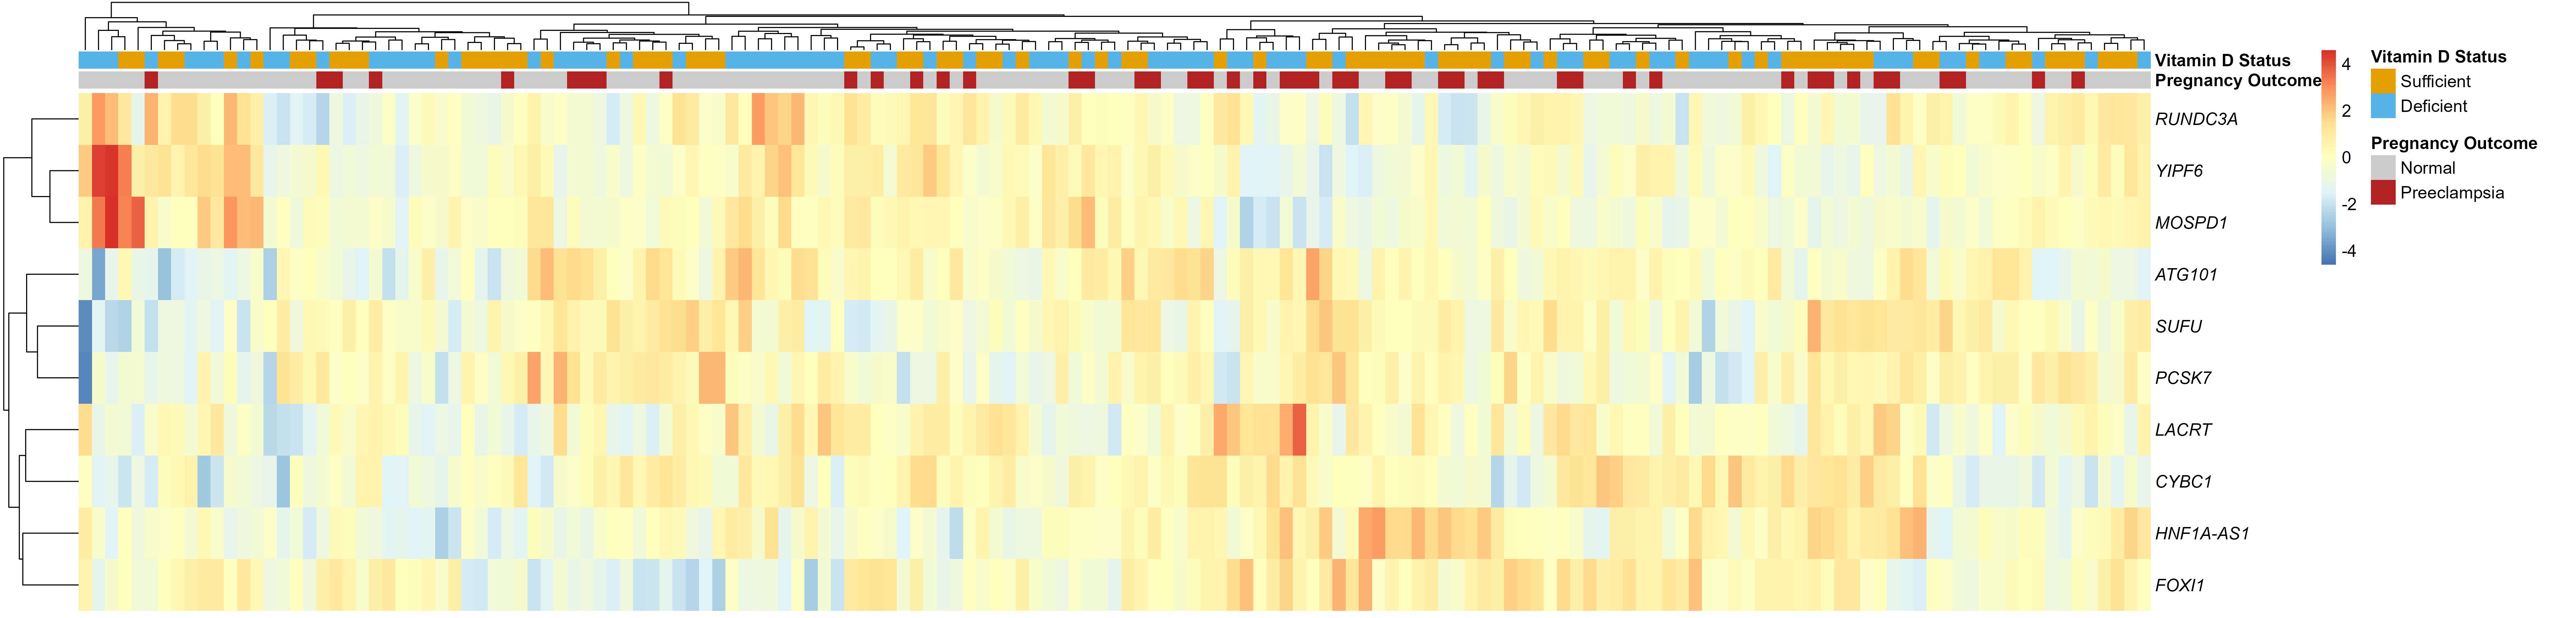
\includegraphics[width=\textwidth]{heatmap.png}
\caption{Heatmap of the ten genes with the smallest p-values comparing preeclampsia and normal pregnancies. Expression is row-scaled (z-score), and genes and samples are clustered by Euclidean distance with complete linkage. Tracking bars show pregnancy outcome and vitamin D status for each woman.}
\label{fig:heatmap}
\end{figure}

\subsection{Gene Screen}
Across all 500 genes, mean differences in expression between preeclampsia and normal pregnancies were small and centered near zero (Figure~\ref{fig:beeswarm}). Fourteen genes had p $<$ 0.05, which is fewer than the approximately 25 genes expected by chance alone across 500 tests, and these genes appeared at both ends of the distribution.

\begin{figure}[htbp]
\centering
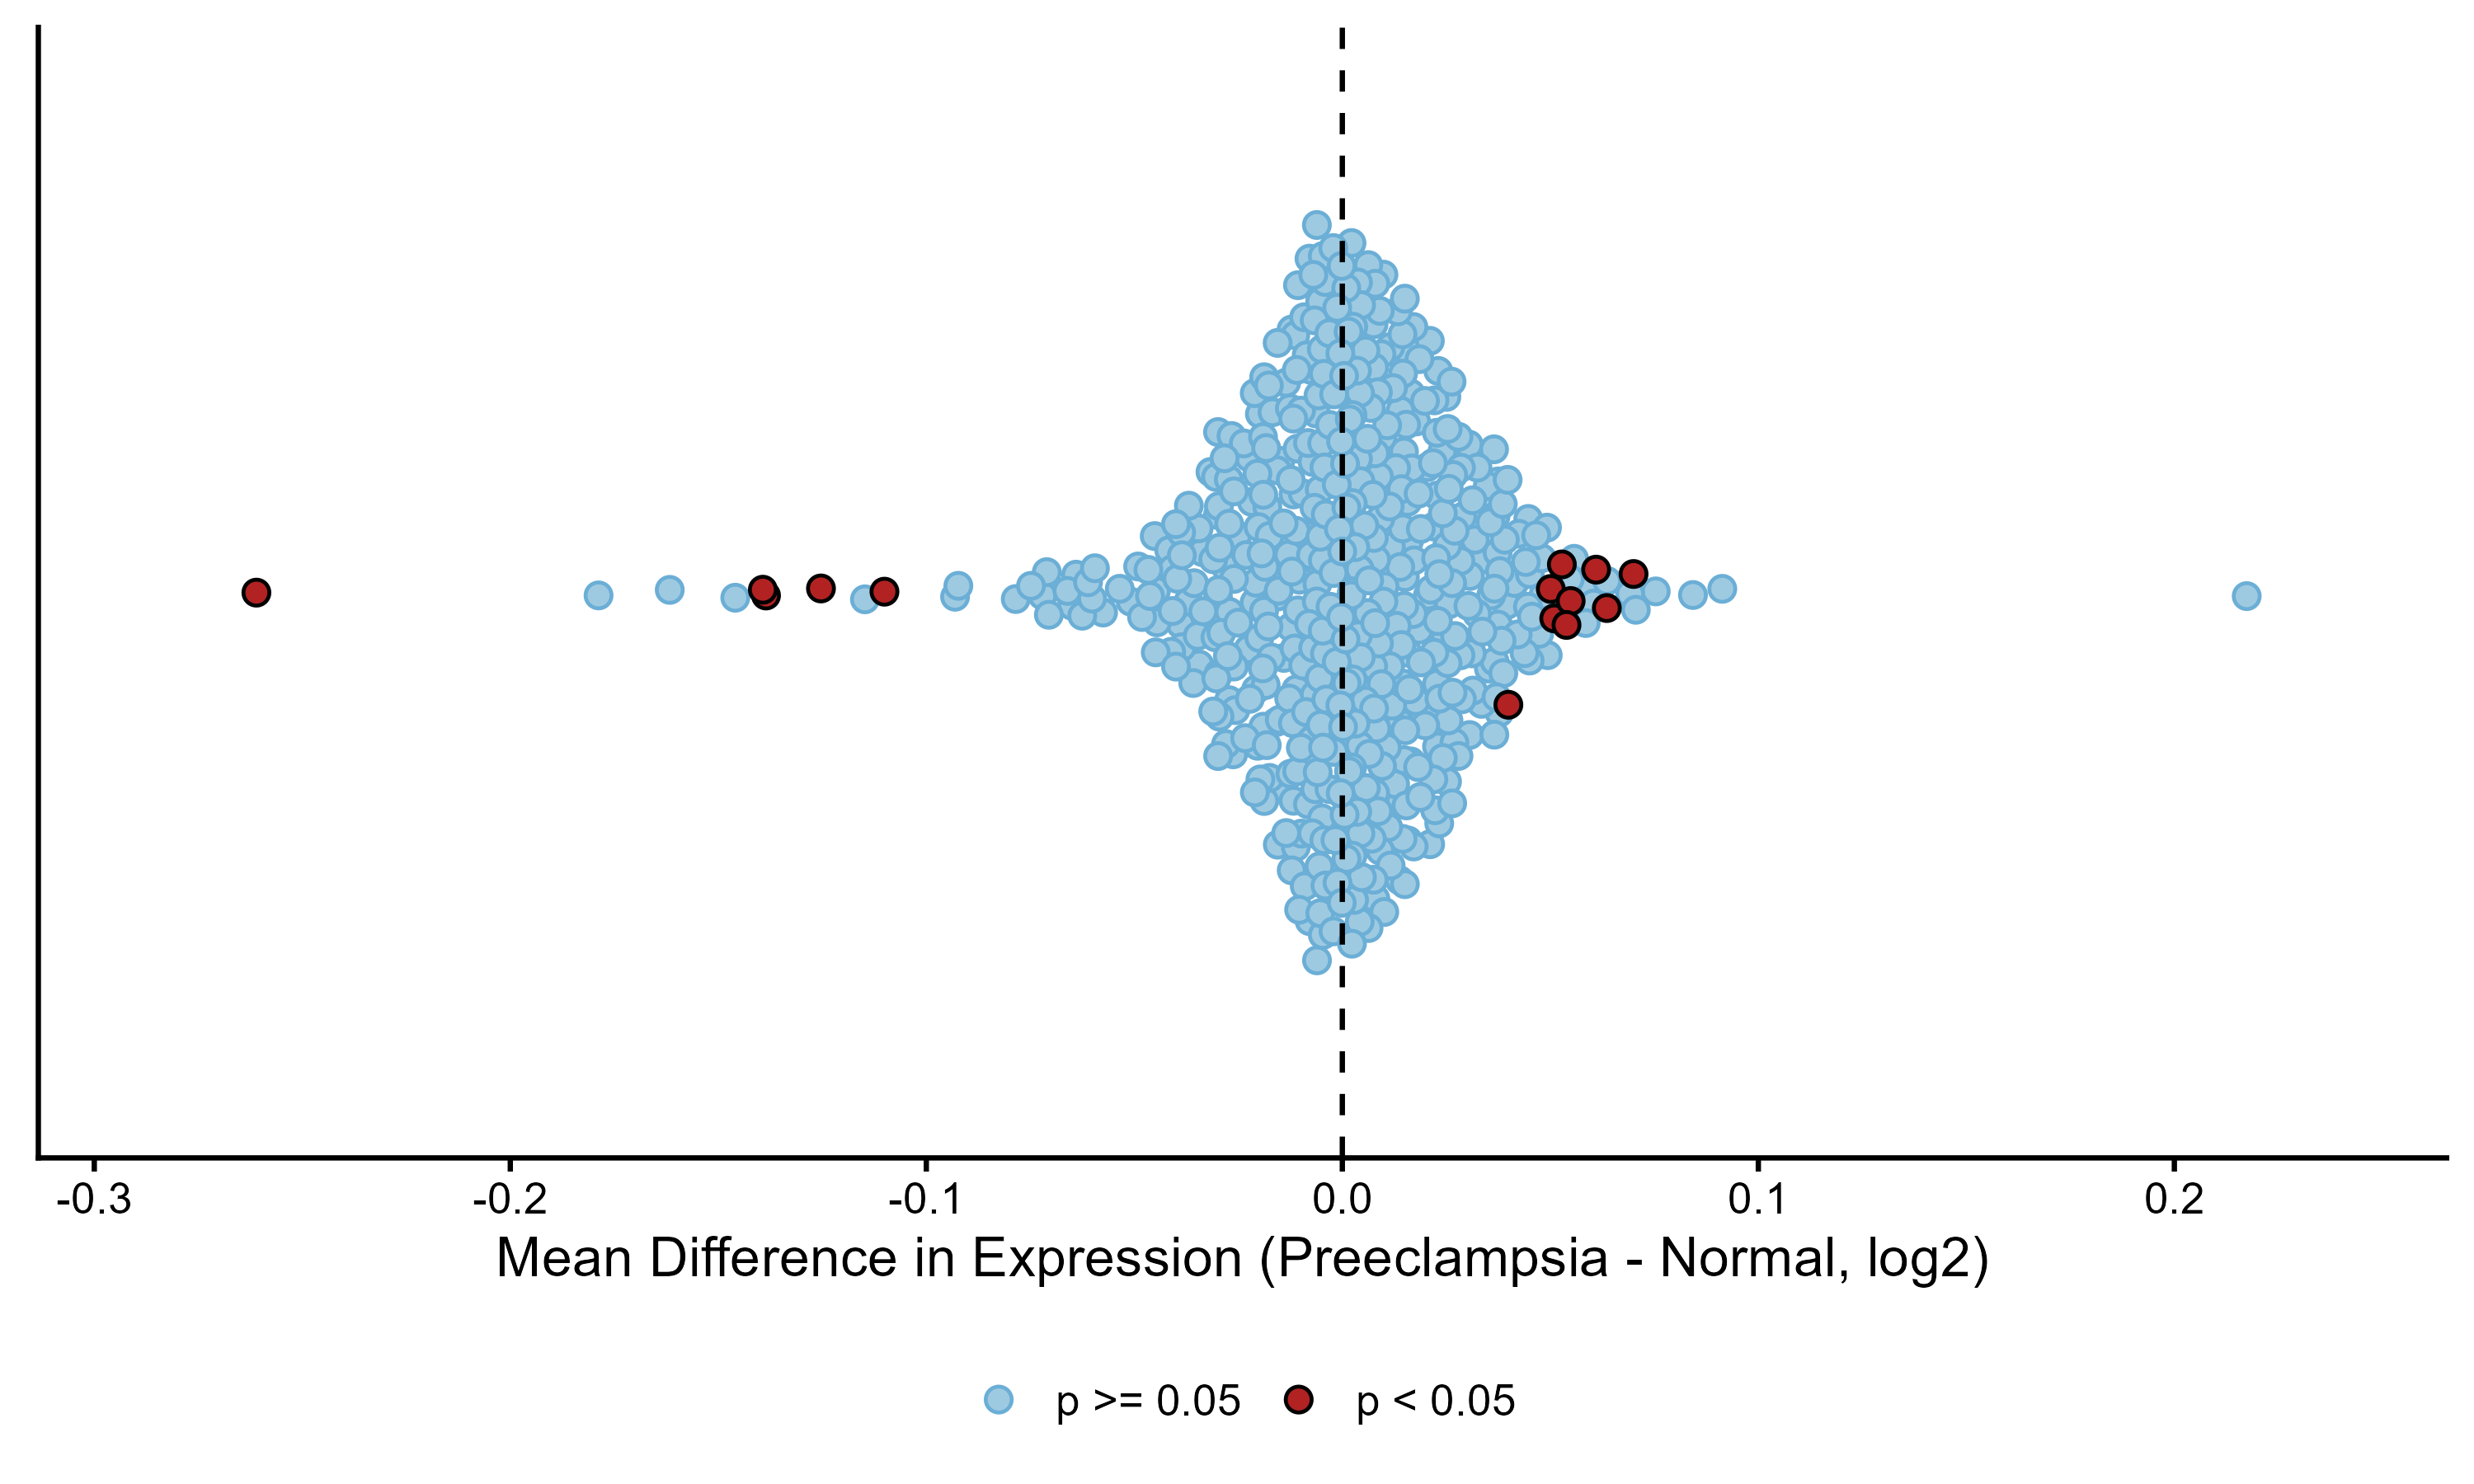
\includegraphics[width=\textwidth]{beeswarm.png}
\caption{Beeswarm plot of the mean difference in log$_2$ expression (preeclampsia minus normal) for all 500 genes. Each point represents one gene, genes with p $<$ 0.05 from Welch's t-test are shown in red, and the dashed line marks no difference.}
\label{fig:beeswarm}
\end{figure}h

\bibliographystyle{plainnat}
\bibliography{references,packages}

\end{document}